\documentclass{cake-classes/short-report-fa}
\usepackage{pdflscape}
\newcommand{\ورب}[1]{\lr{\Verb!#1!}}
\begin{document}
\درج‌عنوان‌سند

\listoffigures

\قسمت{مقدمه}
در این گزارش، جزییات معماری پیشنهادی برای ساخت پروژه رباتیک توسط کاربر و اجرای آن در محیط شبیه‌سازی یا واقعی شرح داده شده است. از آنجایی که کیک یک پروژهٔ کاربر محور است، این سند هم به رابطهٔ سرویس‌ها در پشت صحنه، و هم به نمود آن در تجربهٔ کاربری\پانویس{User Experience (UX)} می‌پردازد.

\قسمت{فرایند ساخت اولین پروژه}

تجربهٔ یک کاربر که برای اولین بار در سیستم لاگین می‌کند، به کمک یک دیاگرام توالی\پانویس{Sequence Diagram} نمایش داده شده است (شکل \رجوع{seq-create-project}).

\begin{figure}
	\centering
	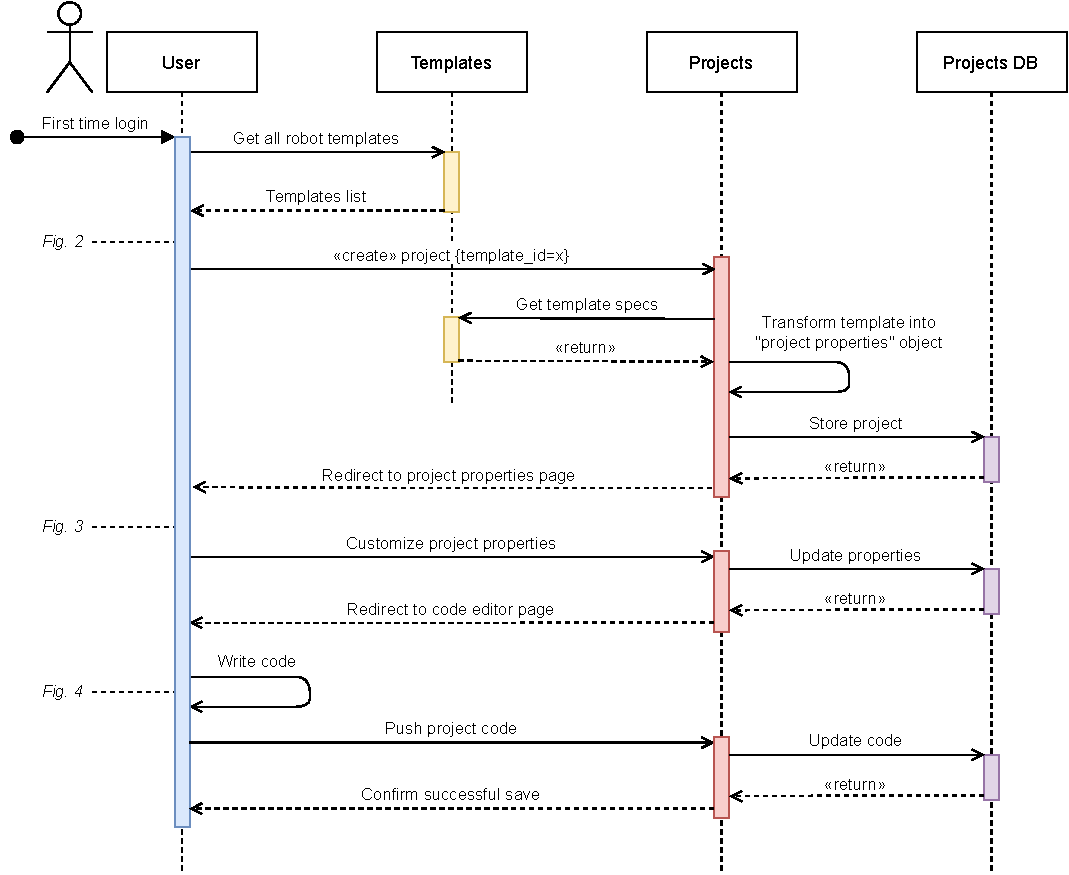
\includegraphics[width=\linewidth]{img/seq-create-project.pdf}
	\شرح{دیاگرام توالی ساخت اولین پروژه}
	\برچسب{seq-create-project}
\end{figure}

\clearpage

همانطور که دیده می‌شود، سناریو با اولین باری که کاربر وارد حساب کاربری خود می‌شود، آغاز می‌شود. همیشه پس از ورود به حساب کاربری، مرورگر به صفحهٔ اصلی پنل ابری هدایت می‌شود اما چون کاربر در اولین ورود به پلتفرم هنوز پروژه‌ای نساخته است، مرورگر او را به صفحهٔ دیگری هدایت می‌کند که در واقع گالری تمپلیت‌های ربات است که محتوای آن از سرویس \مل{Templates} دریافت می‌شود و به صورت شکل \رجوع{templates} به نمایش در می‌آید.

\begin{figure}[h]
	\centering
	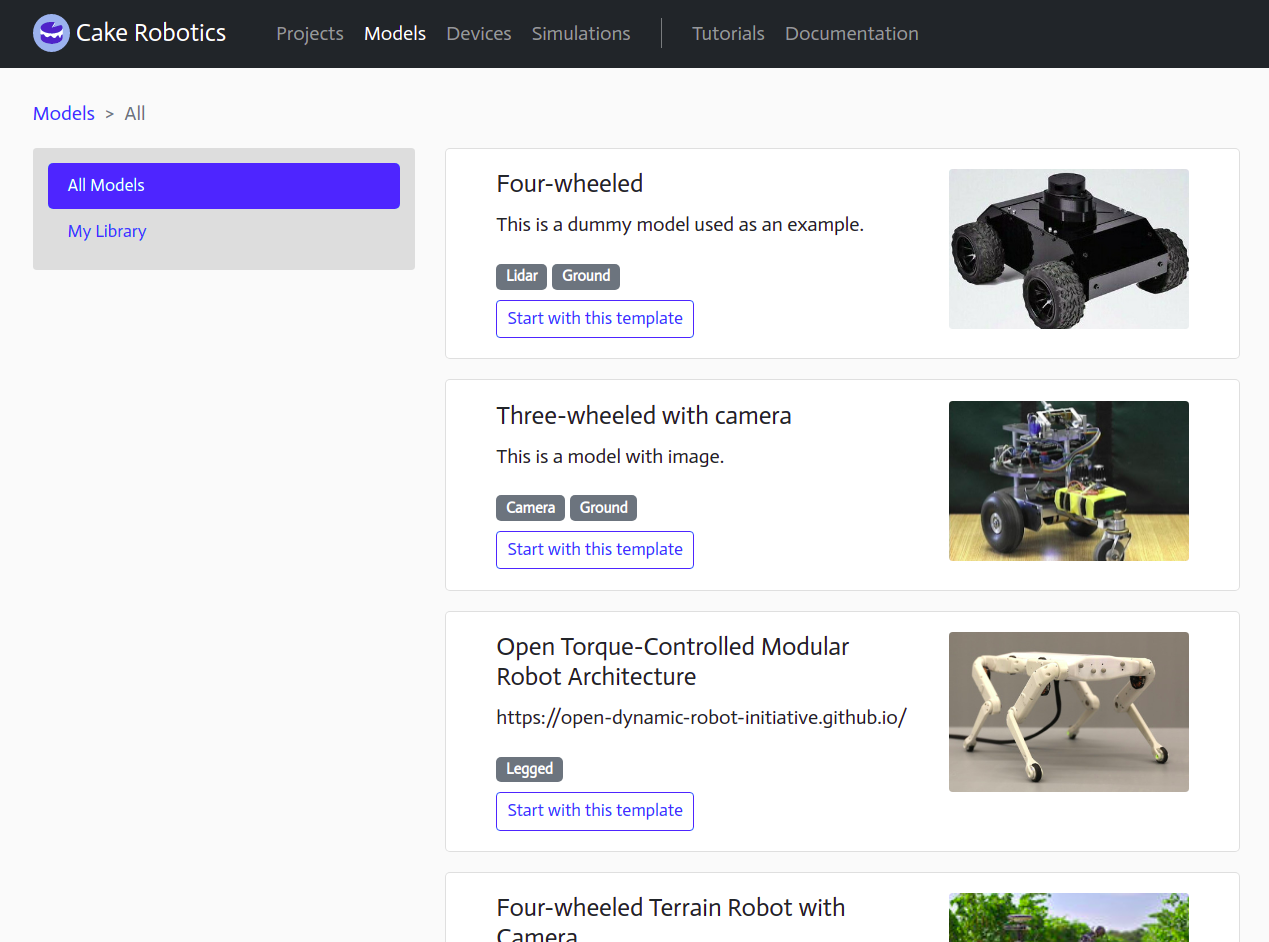
\includegraphics[width=\linewidth]{img/templates.png}
	\شرح{نمای تقریبی صفحهٔ انتخاب تمپلیت ربات}
	\برچسب{templates}
\end{figure}

کاربر با کلیک روی دکمهٔ \مل{Start with this template} درخواستی را به سرویس \مل{Projects} می‌فرستد. در دیاگرام توالی می‌توان اتفاقات پشت صحنه را دید. درخواست کاربر از طریق فرستادن آیدی تمپلیت مورد نظر به سرویس \مل{Projects} آغاز می‌شود.

سرویس \مل{projects} ابتدا تمام اطلاعات تمپلیت را از سرویس \مل{templates} دریافت می‌کند. این اطلاعات در قالب \مل{JSON} منتقل می‌شوند. دقت شود که اینگونه نیست که سرویس \مل{projects} صرفا آیدی تمپلیت را ذخیره کند؛ بلکه این سرویس عملا یک کپی از تمپلیت می‌گیرد و آیدی را فراموش می‌کند. دلیل این امر این است که تمپلیت ممکن است بعدا به روز شود ولی ما نمی‌خواهیم پروژهٔ کاربر که براساس آن تمپلیت ساخته شده است ناخواسته تغییر کند.

اطلاعات تمپلیت پیش از ذخیره شدن در دیتابیس پروژه‌ها، از یک تابع تبدیل گذر می‌کنند. این تابع تبدیل، داده‌ را از تمپلیت به ساختار مشخصات پروژه (\مل{Project Properties}) تبدیل می‌کند. برای مثال، فیلدهایی نظیر «نام تمپلیت» یا «تگ‌ها» حذف می‌شوند و فیلدهایی نظیر «نام پروژه» اضافه می‌شوند. برای دیدن ساختار دقیق تمپلیت، مشخصات پروژه و تابع تبدیل، به مستندات سرویس‌های مربوطه رجوع کنید.

در نهایت، ساختار دادهٔ به دست آمده که نمایندهٔ مشخصات پروژه است، در پایگاه دادهٔ غیررابطه‌ای \مل{Projects DB} ذخیره می‌شود. در دیتابیس، محلی نیز برای آپلود کدها به وجود می‌آید که خارج از ساختار دادهٔ مشخصات است. به بیان دیگر، برای هر پروژه، یک ساختار دادهٔ مشخصات پروژه وجود دارد که به صورت \مل{JSON} قابل نمایش است، و یک فایل کد وجود دارد که به صورت رشته است. در نسخه‌های آتی پشتیبانی از بیش از یک فایل کد باید اضافه شود.

نکته: پروژهٔ خالی ایجاد شده باید در همان لحظه قابل اجرا باشد. به عبارتی، نباید پروژه در حالت غیرمجاز (\مل{Invalid State}) وارد دیتابیس شود. این به این معناست که تمام پارامترها و نام‌ها باید مقدار پیش‌فرض داشته باشند.

پس از ذخیرهٔ پروژه در دیتابیس، کاربر به صفحهٔ تنظیمات پروژه هدایت می‌شود (شکل \رجوع{project-props}). در این صفحه کاربر می‌تواند نام پروژه، درایورهای سخت‌افزاری، پارامترهای هندسی و... را وارد کند. در نسخه‌های اولیه این پارامترها در حدی گسترده نیستند که باعث تغییر ساختار \مل{URDF} شوند و حداکثر پارامترهای عددی آن را تغییر می‌دهند. در این حالت، در واقع \مل{URDF} در تمپلیت وجود داشته و توسط ادمین سایت به طور دستی درست شده است. این بدین معناست که مثلا اگر یک ربات سه چرخ با لیدار داریم، می‌توانیم ابعاد چرخ‌ها، ربات، جرم آنها و حداکثر گشتاور موتورها را تعریف کنیم. حتی تغییر درایور موتورها ممکن است؛ زیرا روی ساختار \مل{URDF} تاثیری ندارد. با این حال، تعریف چرخ جدید، سنسور جدید، مفصل جدید و تغییر شکل از معکب به شش ضلعی ممکن نیست. در نسخه‌های آینده می‌توان این مورد را بهبود داد به گونه‌ای تغییرات پیشرفته‌تری که ساختار \مل{URDF} را نیز تغییر می‌دهند ممکن باشد. این کار ممکن است مستلزم تعریف یک ساختار دادهٔ میانی جدید باشد.

\begin{figure}[h]
	\centering
	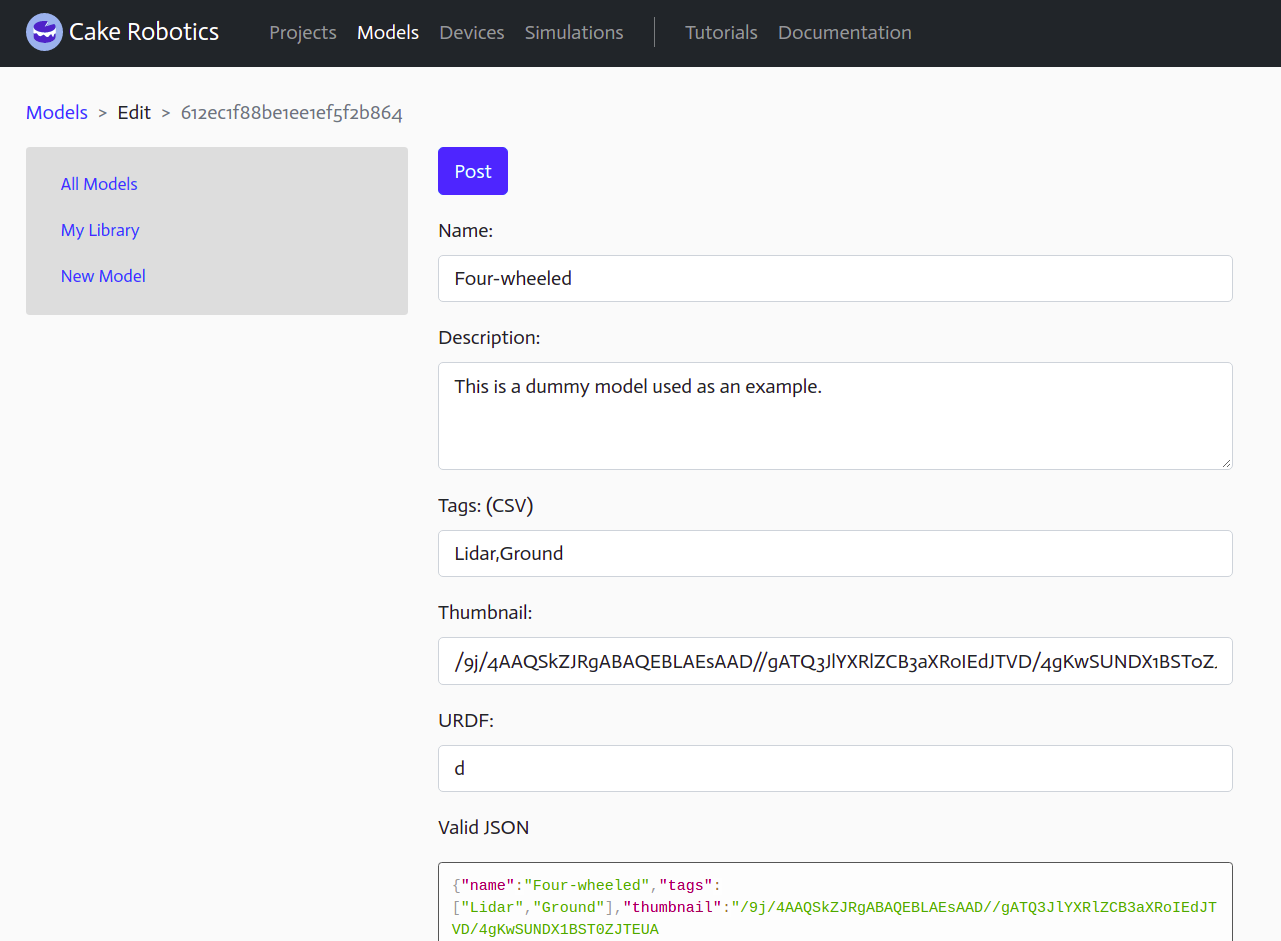
\includegraphics[width=\linewidth]{img/project-props.png}
	\شرح{نمای تقریبی صفحهٔ مشخصات پروژه}
	\برچسب{project-props}
\end{figure}

به هر صورت، هنگامی که کاربر تغییرات را در مشخصات پروژه ایجاد می‌کند، مشخصات جدید را در قالب یک \مل{JSON} به سرویس \مل{Projects} ارسال می‌کند. در پایگاه داده، این مشخصات جایگزین مشخصات قبلی می‌شود. سپس، کاربر به صفحهٔ ویرایش کد هدایت می‌شود.

در صفحهٔ ویرایش کد، یک تابع \مل{main} اولیه وجود دارد که بسیار کوتاه است و یک کار ساده را انجام می‌دهد؛ چیزی شبیه مثال چشمک‌زن آردوئینو. کاربر می‌تواند کد را تغییر دهد و ذخیره کند. شکل \رجوع{code-editor} محیط ویرایش کد را نشان می‌دهد.
 
\begin{figure}[h]
	\centering
	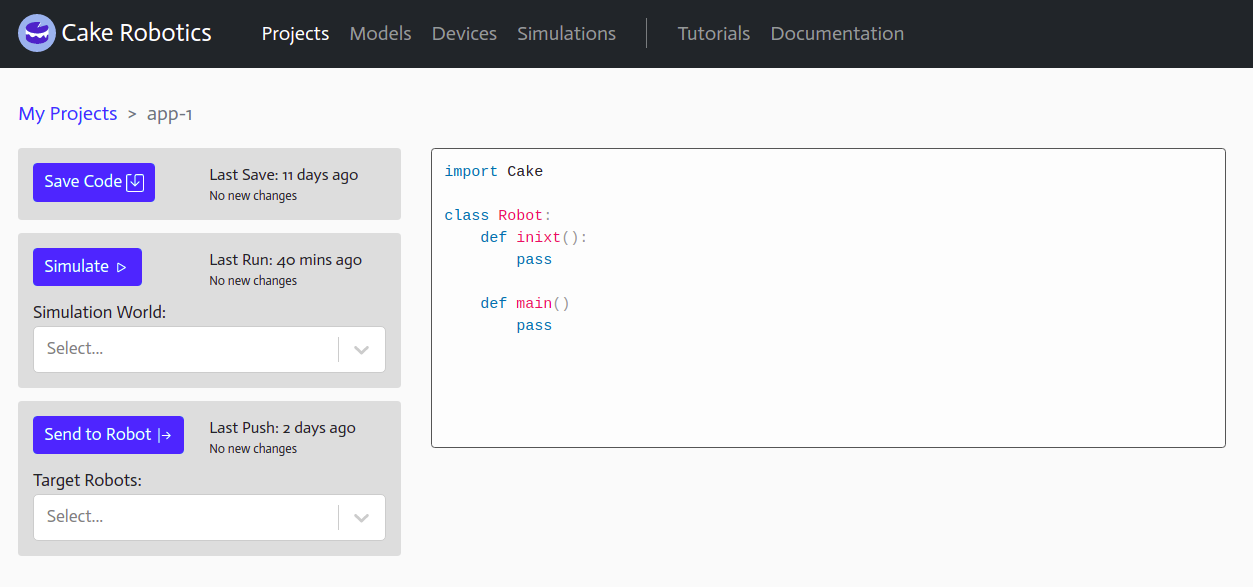
\includegraphics[width=\linewidth]{img/code-editor.png}
	\شرح{نمای تقریبی صفحهٔ ویرایش کد}
 	\برچسب{code-editor}
\end{figure}

\clearpage
\قسمت{فرایند شبیه‌سازی پروژه}

شبیه‌سازی پروژه از صفحهٔ ویرایش کد آغاز می‌شود. کاربر روی دکمهٔ \مل{Start Simulation} کلیک می‌کند. سپس توالی نمایش داده در شکل \رجوع{seq-start-sim} آغاز می‌شود.

\begin{figure}
	\centering
	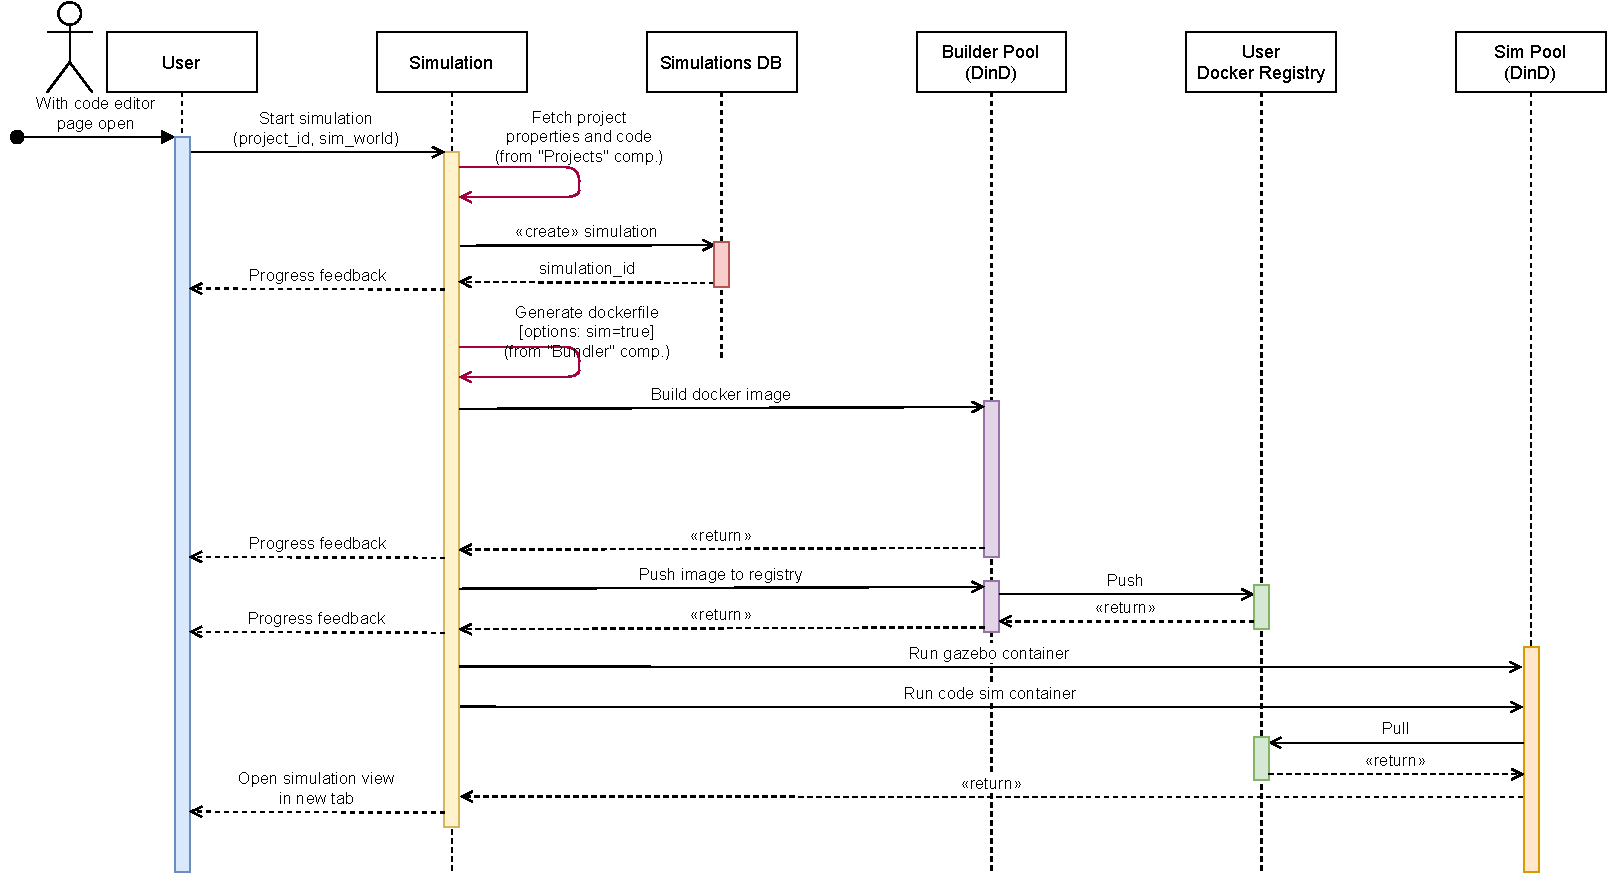
\includegraphics[width=\linewidth]{img/seq-start-sim.pdf}
	\شرح{دیاگرام توالی شبیه‌سازی پروژه}
	\برچسب{seq-start-sim}
\end{figure}

ابتدا سرویس شبیه‌سازی، مشخصات درخواست ایجاد شبیه‌سازی را در دیتابیس ذخیره می‌کند. این کار باعث می‌شود که وضعیت شبیه‌سازی‌های یک پروژه مشخص باشد تا در صورتی که یک شبیه‌سازی در حال اجراست، بتوانیم این امر را در صفحهٔ پروژه نشان دهیم و به جای دکمهٔ \مل{Start Simulation}، دکمه‌های \مل{Open Simulation} و \مل{Stop Simulation} را نشان دهیم. همچنین، می‌توان درصد پیشروی شبیه‌سازی که در حال شروع است را در این دیتابیس نگه داشت تا اگر کاربر صفحه را رفرش کرد بتوان وضعیت را دید. در نهایت، اگر اتفاق ناخواسته‌ای مانند ریستارت شدن سرویس‌ها و... رخ دهد، بازیابی در حالتی که اطلاعات در یک پایگاه داده پایا موجود باشد آسان‌تر است. این پایگاه داده می‌تواند رابطه‌ای و غیررابطه‌ای، همچنین ذخیره‌شده در دیسک یا \مل{RAM} باشد.

پس از ثبت شبیه‌سازی، یک \مل{ID} تولید می‌شود که در مراحل آتی از آن برای برچسب‌زنی و... استفاده می‌شود.

برای شروع شبیه‌سازی لازم است کد کاربر به همراه پیش‌نیازها و... به صورت یک \مل{Dockerfile} درآید. این کار در سرویس \مل{Bundler} انجام می‌شود. این فایل بسیار شبیه به \مل{Dockerfile}ـی است که باید برای ساخت ایمیج برای ربات استفاده شود؛ با این تفاوت که برای ساخت این فایل پارامتر \ورب{sim=true} به \مل{Bundler} ارسال می‌شود. این امر باعث می‌شود \مل{Bundler} پیش از آغاز ساخت \مل{Dockerfile}، مشخصات ربات را از یک تبدیل مخصوص گذر دهد. در این تبدیل، تمام درایورهای سخت‌افزاری تعریف شده در مشخصات حذف شده و با درایورهای شبیه‌سازی جایگزین می‌شوند. این درایورهای شبیه‌سازی، به جای خواندن تاپیک‌های سخت‌افزاری \مل{ROS} و نوشتن آن‌ها روی سخت‌افزار، آن‌ها را روی \مل{ROS Bridge} می‌نویسند و به طور مشابه، اطلاعات سنسور را از \مل{ROS Bridge} می‌خوانند. این امر باعث می‌شود ارتباط با کانتینر شبیه‌ساز (که خارج از کانتینر کد کاربر است) ممکن شود. معماری خروجی نهایی که در پایان این توالی به دست می‌آید، به صورت شکل \رجوع{sim-containers} است.

\begin{figure}
	\centering
	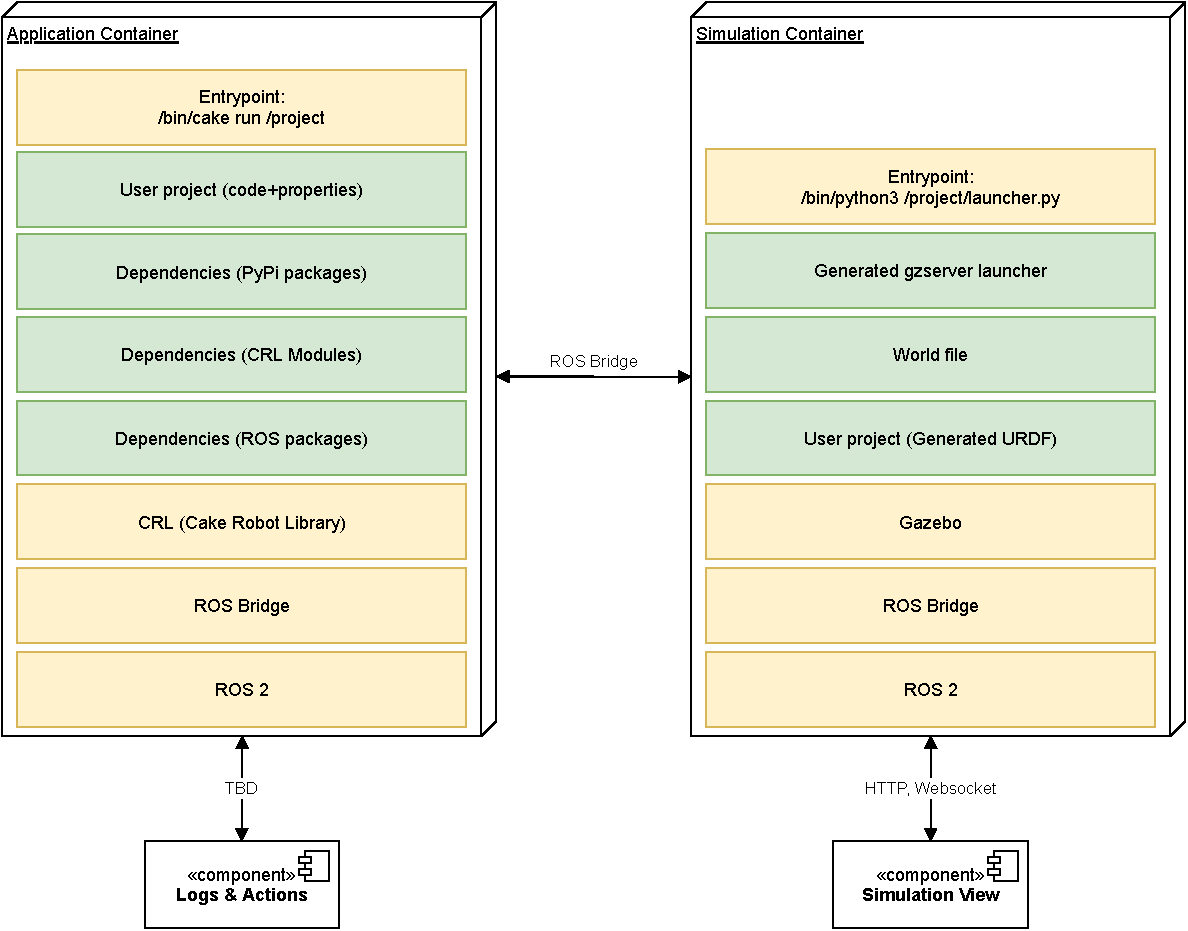
\includegraphics[width=\linewidth]{img/sim-containers.pdf}
	\شرح{دیاگرام کانتینرهای داکر که برای شبیه‌سازی یک پروژه ساخته و اجرا می‌شوند}
	\برچسب{sim-containers}
\end{figure}

\قسمت{فرایند ارسال پروژه به ربات واقعی}

این فرایند تا حدودی مشابه فرایند آغاز شبیه‌سازی است؛ بنابراین از تکرار توضیحات صرف نظر شده است و تنها به آوردن دیاگرام توالی (شکل \رجوع{seq-push-to-robot}) اکتفا شده است.

\begin{landscape}
\begin{figure}
	\centering
	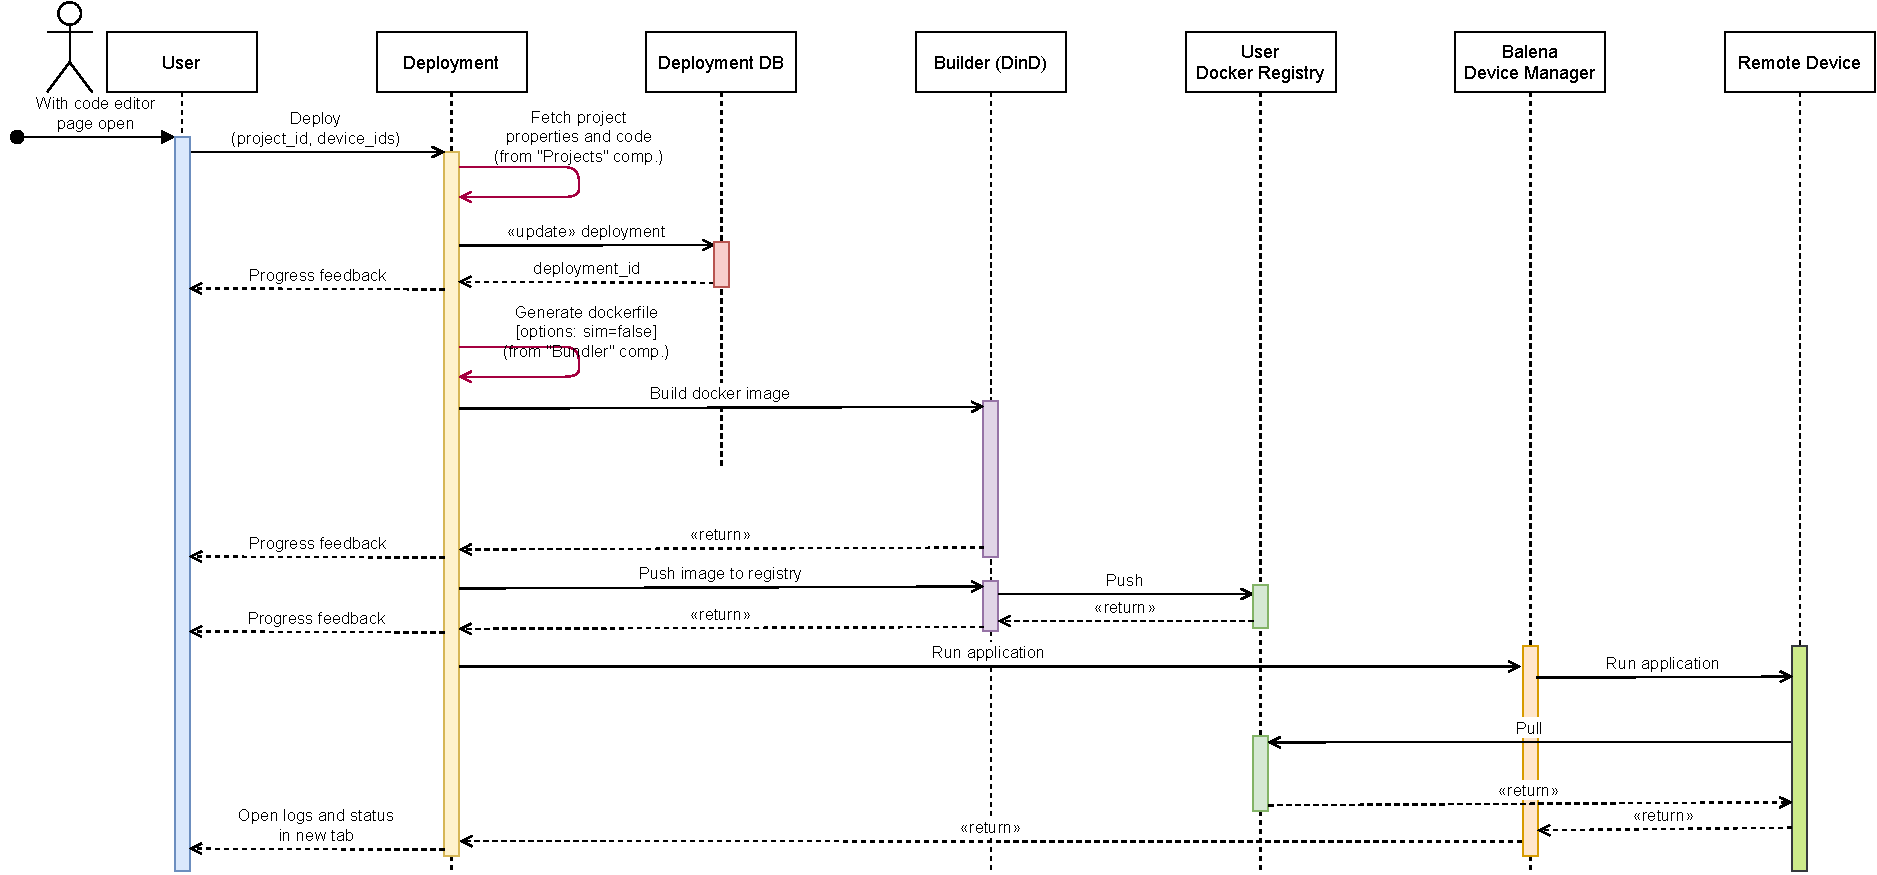
\includegraphics[width=\linewidth]{img/seq-push-to-robot.pdf}
	\شرح{دیاگرام توالی اجرای کد در ربات واقعی}
	\برچسب{seq-push-to-robot}
\end{figure}
\end{landscape}

\end{document}
